%% Copyright 1998 Pepe Kubon
%%
%% `two.tex' --- 2nd chapter for thes-full.tex, thes-short-tex from
%%               the `csthesis' bundle
%%
%% You are allowed to distribute this file together with all files
%% mentioned in READ.ME.
%%
%% You are not allowed to modify its contents.
%%

%%%%%%%%%%%%%%%%%%%%%%%%%%%%%%%%%%%%%%%%%%%%%%%%%
%
%     Chapter 3
%
%%%%%%%%%%%%%%%%%%%%%%%%%%%%%%%%%%%%%%%%%%%%%%%%

\chapter{Bilingual Language Models}
\label{two}

In phrase-based statistical machine translation (SMT), the decoder (Section~\ref{intro-decoder}) breaks down a source sentence into phrases and translates one source phrase at a time. For each source phrase, the decoder uses a translation model (Section~\ref{intro-tm}) to get the corresponding target phrase. To model the target language fluency, it also uses a language model (Section~\ref{intro-lm}). A log-linear combination of these models along with additional features are used to score each hypothesis. The decoder then searches for a path in the search tree which gives the highest hypothesis score for the final translation.

As stated in section~\ref{intro-bilm}, during the decoding process, information from source words outside the current phrase pair in consideration is available indirectly through target words which are translations of these source, if those target words are close enough to affect the language model scores. Due to this, the translation of each source phrase is performed in isolation without significant information from other source words in the sentence. The effect can be seen in the following example:

\begin{figure}[htbp]
	\begin{center}
		Maria no daba una bofetada a la burja verde
	\end{center}
\end{figure}

For this sentence we would get the following phrase segmentations: \textit{Maria no, daba una bofetada a la, bruja verde}. Here, the translation of \textit{Maria no} is not affected by the source words \textit{daba} or \textit{bofetada} or \textit{bruja}. The other possible segmentation could be as shown in Table~\ref{table:sample-phrase-table-entry}. The translation of words \textit{Maria no daba una bofetada a la} can be done using the phrases \textit{Maria no, daba una bofetada a la} or \textit{Maria, no, daba una bofetada, a la}. The decoder cannot make use of the fact that both these options lead to the same translation \textit{Mary did not slap the}. If the first option is chosen, the translation of \textit{no} is affected by \textit{Maria}, but in the second option, \textit{no} is only affected by \textit{Maria} via the language model.

To introduce the effect of source words outside the current phrase pair in consideration, considerable amount of work has been done in the past. In this thesis, we extend the work of \cite{Niehues2011} and \cite{Stewart2014} to create \textit{bilingual language models (Bi-LMs)} that will be used as additional features to the decoder.

\section{What are Bilingual Language Models?}
Bi-LMs are n-gram language models which are trained on bitokens instead of simple word tokens as done for standard language models (Section~\ref{intro-lm}). Bitokens are generated using the source and target sentences from the parallel corpora and their alignments. To understand what bitokens are, let us look at two parallel sentences shown in Fig.~\ref{fig:bitoken-sentences}:

\begin{figure}[htbp]
	\begin{center}
		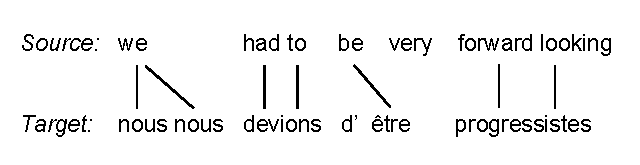
\includegraphics[width=10cm]{files/images/bitoken-example}
	\end{center}
	\caption{Source and target sentences with their alignments for creating bitokens \cite{Stewart2014}}
	\label{fig:bitoken-sentences}
\end{figure}

Using the parallel sentences and their alignments shown above we will create a bitoken sequence. When creating hte bitokens, we want to make sure that all the target words are used. In the exmample above, the source word \textit{we} is aligned to target words \textit{nous nous}. We will replicate \textit{we} twice and align both \textit{nous} with both the \textit{we} to create the bitokens \textit{we-nous} and \textit{we-nous}. Next we have the source words \textit{had to} aligned to \textit{devions}. We will join \textit{had} and \textit{to} to create a single token \textit{had\_to} and align that to \textit{devions} to get \textit{had\_to-devions}. Since, the target word \textit{d'} is not aligned to any source word, we align it to \textit{NULL} and create a bitoken \textit{NULL-d'}. For the source word \textit{very}, as it is not aligned to any target word, it is dropped. Similarly, we also get the bitoken \textit{forward\_looking-progressistes}. The final bitokens are shown in Fig.~\ref{fig:bitokens}:

\begin{figure}[htbp]
	\begin{center}
		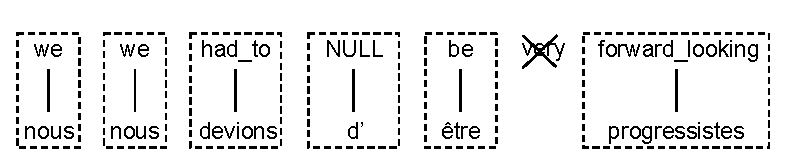
\includegraphics[width=10cm]{files/images/bitoken-example2}
	\end{center}
	\caption{Bitokens created from the parallel sentences and their alignments shown in Fig.~\ref{fig:bitoken-sentences}}
	\label{fig:bitokens}
\end{figure}

More formaly, given a pair of sentences $e_1^I = e_1 ... e_I$, $f_1^J = f_1 ... f_J$ and alignments $A=\{(i, j)\}$, the bitokens are:
\begin{eqnarray}
	b_j = \{f_j\} \cup \{e_i | (i, j) \in A\}
\end{eqnarray}

This makes sure that the number of bitokens $b_j$ are equal to the number of target words. These bitoken sequences can then be used to create a language model called bilingual language model, formalized as follows:

\begin{eqnarray}\label{eqn:bitoken}
p(e_1^I, f_1^J, A) = \prod_{j=1}^J P(b_j | b_{j-1}...b_{j-n})
\end{eqnarray}

The advantage of using Bi-LMs is that they can be used in phrase-based SMT as additional features in the log linear model. When the decoder scores each hypothesis using scores from translation and language model, it can easily incorporate the probability from Eqn.~\ref{eqn:bitoken}. Even though, Bi-LMs are language models, but they act more as translation models as they do not model the fluency of target language but model the translation of source words.

In Bi-LMs the bitoken vocabulary size increases by many folds compared to the vocabulary size of target words. For example, as shown by \cite{Stewart2014}, the target word \textit{être} might be split into multiple bitokens: \textit{be-être}, \textit{being-être} and \textit{to\_be-être}. This large vocabulary also leads to an increase in the sparsity in data for language modelling. Table~\ref{table:vocab-comparison} shows the number of bitokens compared to the number of target words in our corpus. We will explain in detail about our data and alignments used to create the bitokens in Chapter~\ref{three}. 

\begin{table}
	\begin{center}
		\begin{tabular}{|c|c|}
			\hline
			\textbf{Number of Target Words} & \textbf{Number of Bitokens}\\\hline
			152318 & 3827728\\\hline
		\end{tabular}
		\caption{Number of target words vs number of bitokens in our data}
		\label{table:vocab-comparison}		
	\end{center}
\end{table}

%In the next section we discuss the method adopted to handle the large bitoken vocabulary.

%\section{Tackling Sparsity in Language Models}
%In the previous section we see that bitokens have a larger vocabulary than the target language vocabulary of the training data. 
To tackle the problem of large vocabulary and sparsity, \cite{Niehues2011} introduced coarse Bi-LMs. When training LMs and Bi-LMs, if the words are replaced by some word class to reduce the vocabulary size, they are then called \textit{Coarse LMs/Bi-LMs}. When creating Bi-LMs, \cite{Niehues2011} replaced both the source and target words in their Arabic>English SMT with the corresponding Part-of-Speech tags. \cite{Stewart2014} extended this idea and replaced both source and target words with cluster ids generated using \textbf{mkcls} \cite{Och1995}. \cite{Stewart2014} not only clustered the initial source and target words, but also experimented with clustering the bitokens too. Figure~\ref{fig:bitokens-clusters} shows the 3 ways of creating bitoken sequences for Bi-LMs:
\begin{itemize}
	\item Word Clustering: Create bitoken sequences with only source and target word cluster ids. The bitokens are then used to create Bi-LMs.
	\item Bitoken Clustering 1: Create bitokens without clustering source and target words. Cluster the bitokens and then use the bitoken sequences augmented with bitoken cluster ids to create Bi-LMs.
	\item Bitoken Clustering 2: Create bitoken sequences with source and target word cluster ids. Cluster the bitoken sequences and then use the bitoken sequences with bitoken cluster ids to create Bi-LMs.
\end{itemize}

\begin{figure}[htbp]
	\begin{center}
		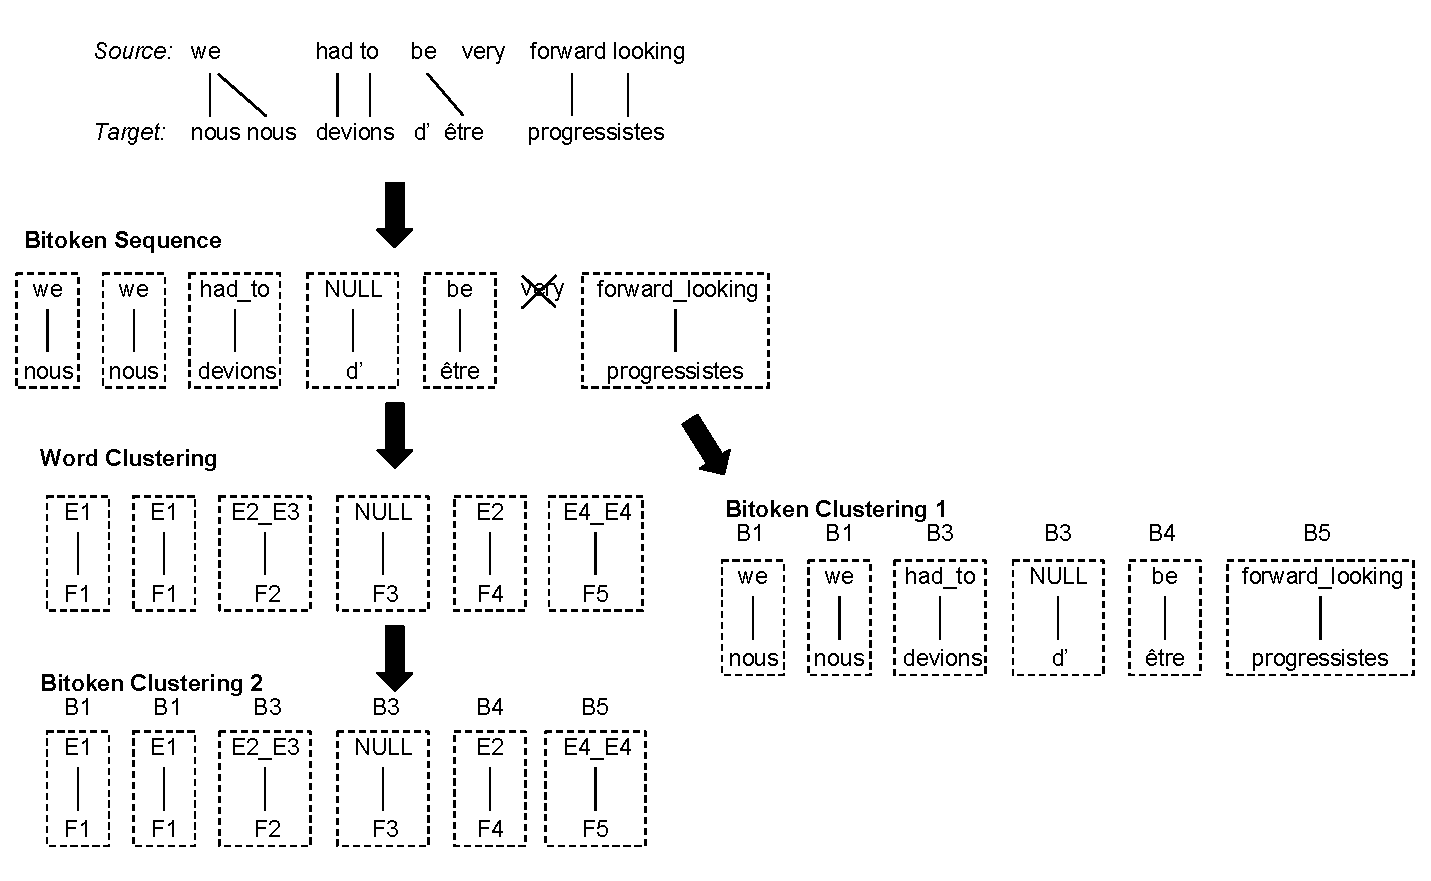
\includegraphics[width=15cm]{files/images/bitoken-example3}
	\end{center}
	\caption{Creating bitokens, word clusters and bitoken clusters \cite{Stewart2014}}
	\label{fig:bitokens-clusters}
\end{figure}

\cite{Ammar2013,Bisazza2014} showed that coarse LMs along with the standard LM are particularly effective for morpholigically rich languages. Motivated by this, \cite{Stewart2014} used a combination of coarse LMs and coarse Bi-LMs in their experiments, which are as follows:
\begin{itemize}
	\item Coarse LM created by augmenting the target language corpus with word cluster ids of size 100. (Coarse LM $100_{tgt}$)
	\item Coarse LM created by augmenting the target language corpus with word cluster ids of size 100. (Coarse LM $1600_{tgt}$)
	\item Augment the source and target language corpus with word cluster ids of size 400 and 400 respectively. This augmented corpus along with their alignments was used to create bitoken sequences. These bitoken sequences were used to create the following two coarse Bi-LMs:
	\begin{itemize}
		\item Use the bitoken sequences to train a coarse Bi-LM. (Coarse Bi-LM $(400_{src},\ 400_{tgt})$)
		\item Cluster the bitoken sequences to get bitoken cluster ids of size 400. Augment the corpus using these bitoken cluster ids to create clustered bitoken sequences. Use these sequences to train a coarse Bi-LM. (Coarse Bi-LM $400_{bi}(400_{src},\ 400_{tgt})$).
	\end{itemize}
\end{itemize}

Figure~\ref{fig:baseline} shows in detail the steps taken by \cite{Stewart2014} to create coarse LM and coarse Bi-LMs. The four coarse LMs and Bi-LMs are then used as additional features in phrase-based SMT. We use this system as a baseline to compare with our results. For our work, we used Moses decoder \cite{Koehn2007Moses} and added additional stateful feature functions to use these coarse LMs and Bi-LMs. Also, to create the LMs and Bi-LMs we used \textbf{SRILM}~\cite{Srilm}.

\begin{figure}[htbp]
	\begin{center}
		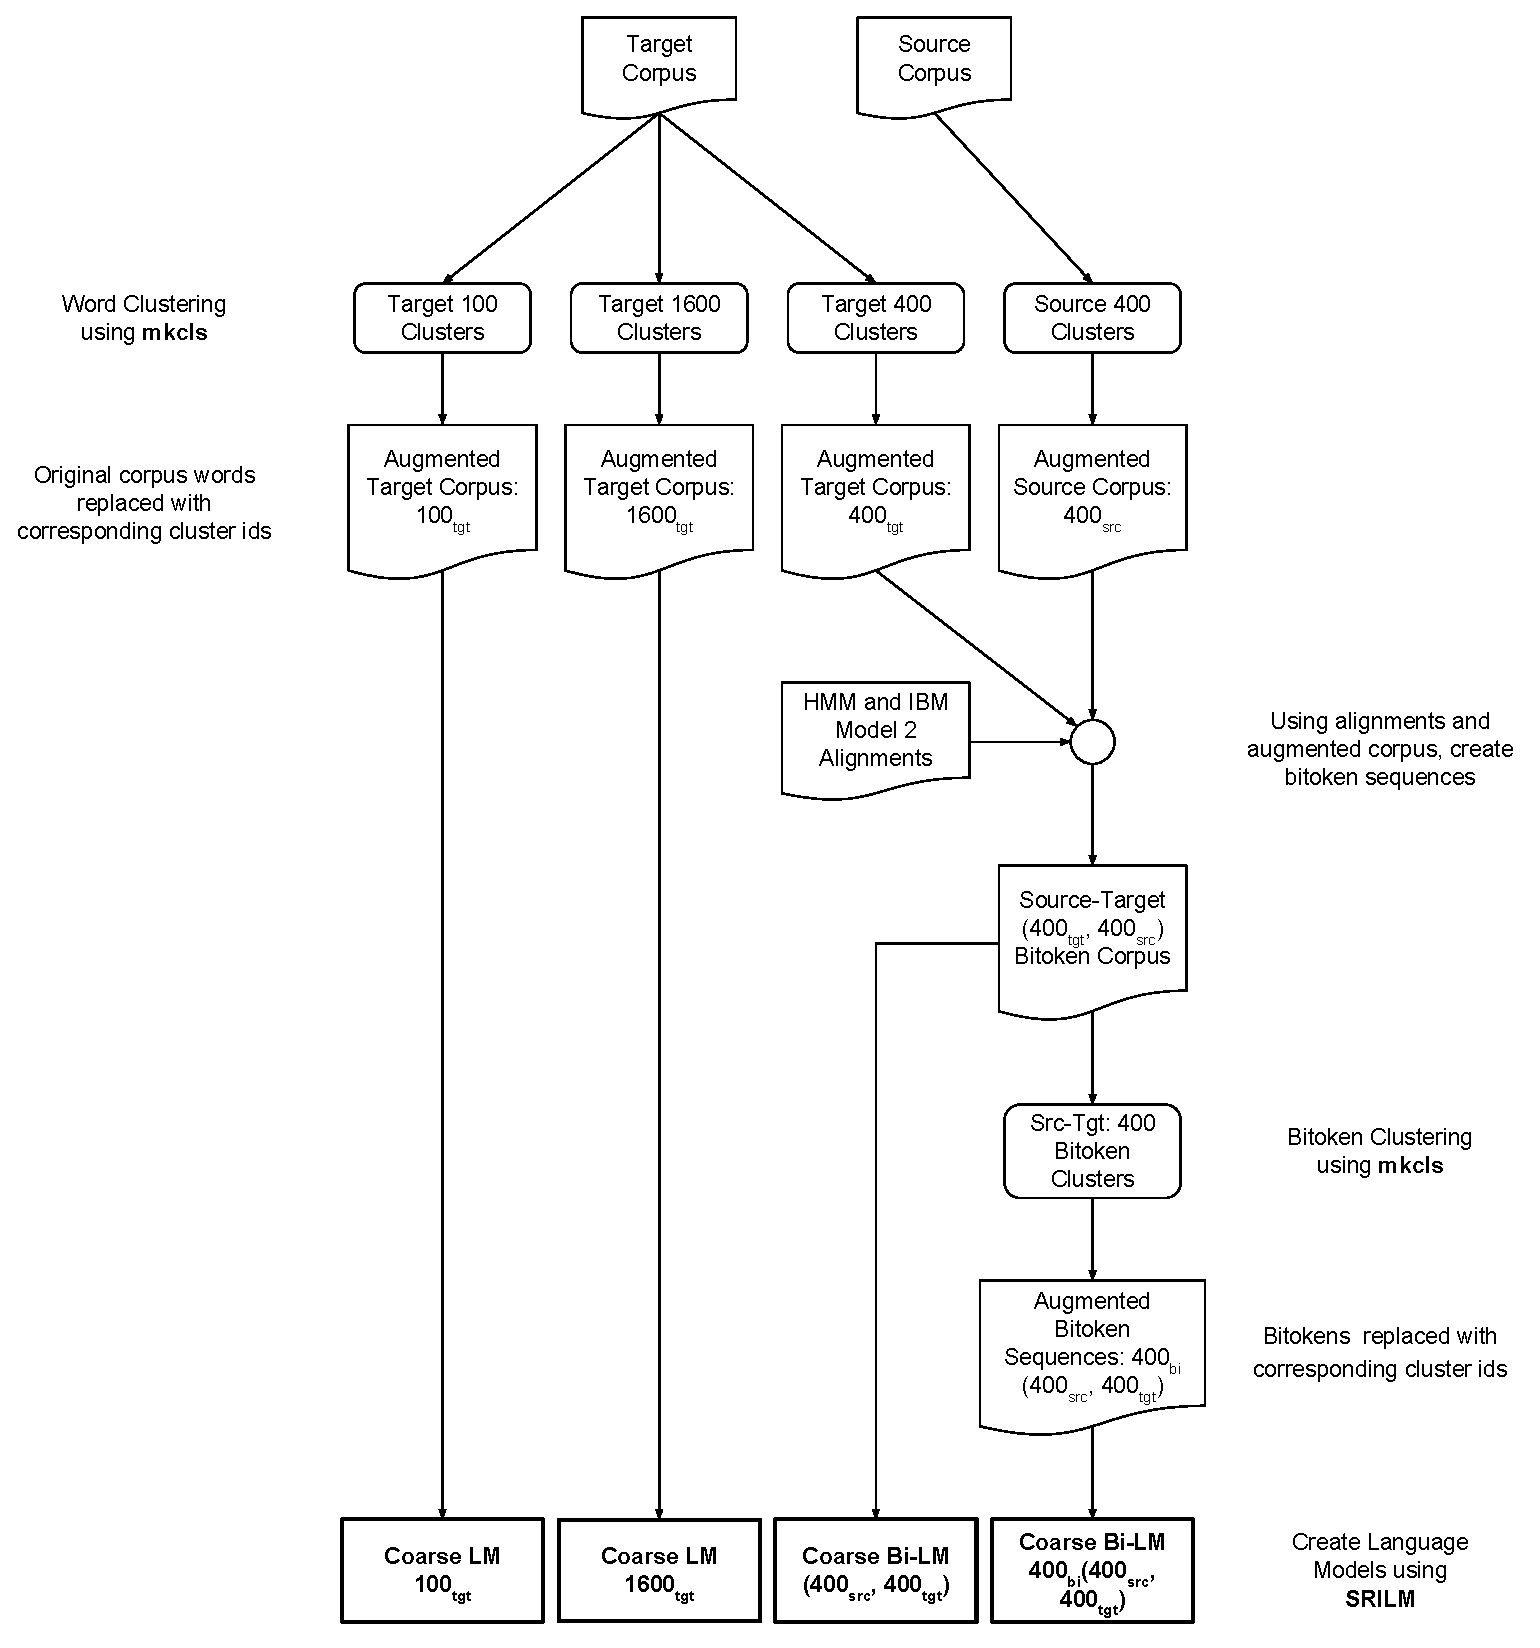
\includegraphics[width=\textwidth]{files/images/baseline}
	\end{center}
	\caption{Creating coarse LMs and coarse Bi-LMs \cite{Stewart2014}}
	\label{fig:baseline}
\end{figure}

In this thesis we extend the work of \cite{Stewart2014} to improve coarse LMs and Bi-LMs. In the next section, we describe in detail the contribution of this thesis, that is, using word embeddings to improve coarse LMs and Bi-LMs.

\section{Bi-LMs using Word Embeddings}
\textbf{mkcls}~\cite{Och1995} is one of the most widely used word clustering toolkit. Motivated by Brown Clustering \cite{Brown1992}, \textbf{mkcls}\footnote{Understanding \textbf{mkcls} by Dr. Chris Dyer: \url{http://statmt.blogspot.ca/2014/07/understanding-mkcls.html}} implements an ensemble of optimzers and merges their results to cluster words into the provided number of classes. \textbf{mkcls} can only cluster monolingual corpus and it performes strongly in that aspect \cite{Blunsom2011}.

The main goal of Bi-LMs is to add more information about source words that are not in the current phrase pair. But current state of the art coarse Bi-LMs only depend on alignments and monolingual word clusters to add more information about source words. For example, the English word \textit{lake} and Chinese word \textzh{潭} \textit{(deep pond)}, which are not direct translations of each other, won't be captured by alignments and hence won't be influencing the coarse Bi-LMs until unless \textbf{mkcls} assigns \textzh{潭} and another Chinese word which is a direct translation of \textit{lake} to the same cluster. To increase the probability that words in Chinese which are semantically similar to \textit{lake} and possibly direct translations get clubbed together in a cluster, we utilize bilingual word embeddings to create the coarse Bi-LMs.

\subsection{Using Word Embeddings to create Bi-LMs}\label{approaches}
In Chapter~\ref{wordvizChapter}, we mention that we utilize \cite{Hermann14} to create bilingual word embeddings for the words in our sentence aligned parallel corpus. To create coarse LMs and Bi-LMs, as done by \cite{Stewart2014}, we need to cluster these embeddings. As mentioned earlier, in our baseline system, we used \textbf{mkcls} to cluster the words in our parallel corpus. To cluster word embeddings, we used \textbf{greedo}~\cite{Stratos2014}, a bottom-up hierarchical clustering algorithm for clustering low-dimensional representation of words under the \cite{Brown1992} model. \cite{Stratos2014} show that the clusters created by \textbf{greedo} recovers clusters which are of comparable quality to the algorithm of \cite{Brown1992}. Using \textbf{greedo} gives us the opportunity to compare our approach to the baseline system without any modifications to the number of clusters because \textbf{mkcls} is also creates Brown clusters.

To use the embeddings and their clusters for creating coarse LMs and coarse Bi-LMs, we propose three approaches.

\subsubsection{Approach 1}\label{approach1}
Once we create the bilingual word embeddings, we can then use them to create the LMs. Figure~\ref{fig:idea1} shows the steps that we took to create our coarse LMs and Bi-LMs. As we did in the baseline, we had clustered the corpora using \textbf{mkcls}, but now we cluster the bilingual word embeddings using \textbf{greedo} to create the following clusters:

\begin{itemize}
	\item Cluster the target language embeddings into clusters of size 100, 400 and 1600.
	\item Cluster the source language embeddings into cluster of size 400. 
\end{itemize}

Using the target language embedding clusters of size 100 and 1600, we augment the target language corpus by replacing the words with their cluster ids. This augmented data is then used to create coarse LMs \textit{Coarse LM $100_{tgt}$} and \textit{Coarse LM $1600_{tgt}$} correspondingly using the language modelling toolkit \textbf{SRILM}.

Using the clusters of size 400 for Target and Source, we augment the parallel corpus by replacing the words with their cluster ids. Using the alignments between the source and target words on the original parallel corpus, we create bitoken sequences. \textit{Coarse Bi-LM $(400_{src},\ 400_{tgt})$} is estimated using the bitoken sequences. The bitoken sequences are further clustered to reduce the vocabulary using \textbf{mkcls}. The size of the cluster in this case is also 400 as done in the baseline system. The bitokens in bitoken sequences are replaced with the new cluster ids. This augmented bitoken sequences is finally used to estimate \textit{Coarse Bi-LM $400_{bi}(400_{src},\ 400_{tgt})$}.

\begin{figure}[htbp]
	\begin{center}
		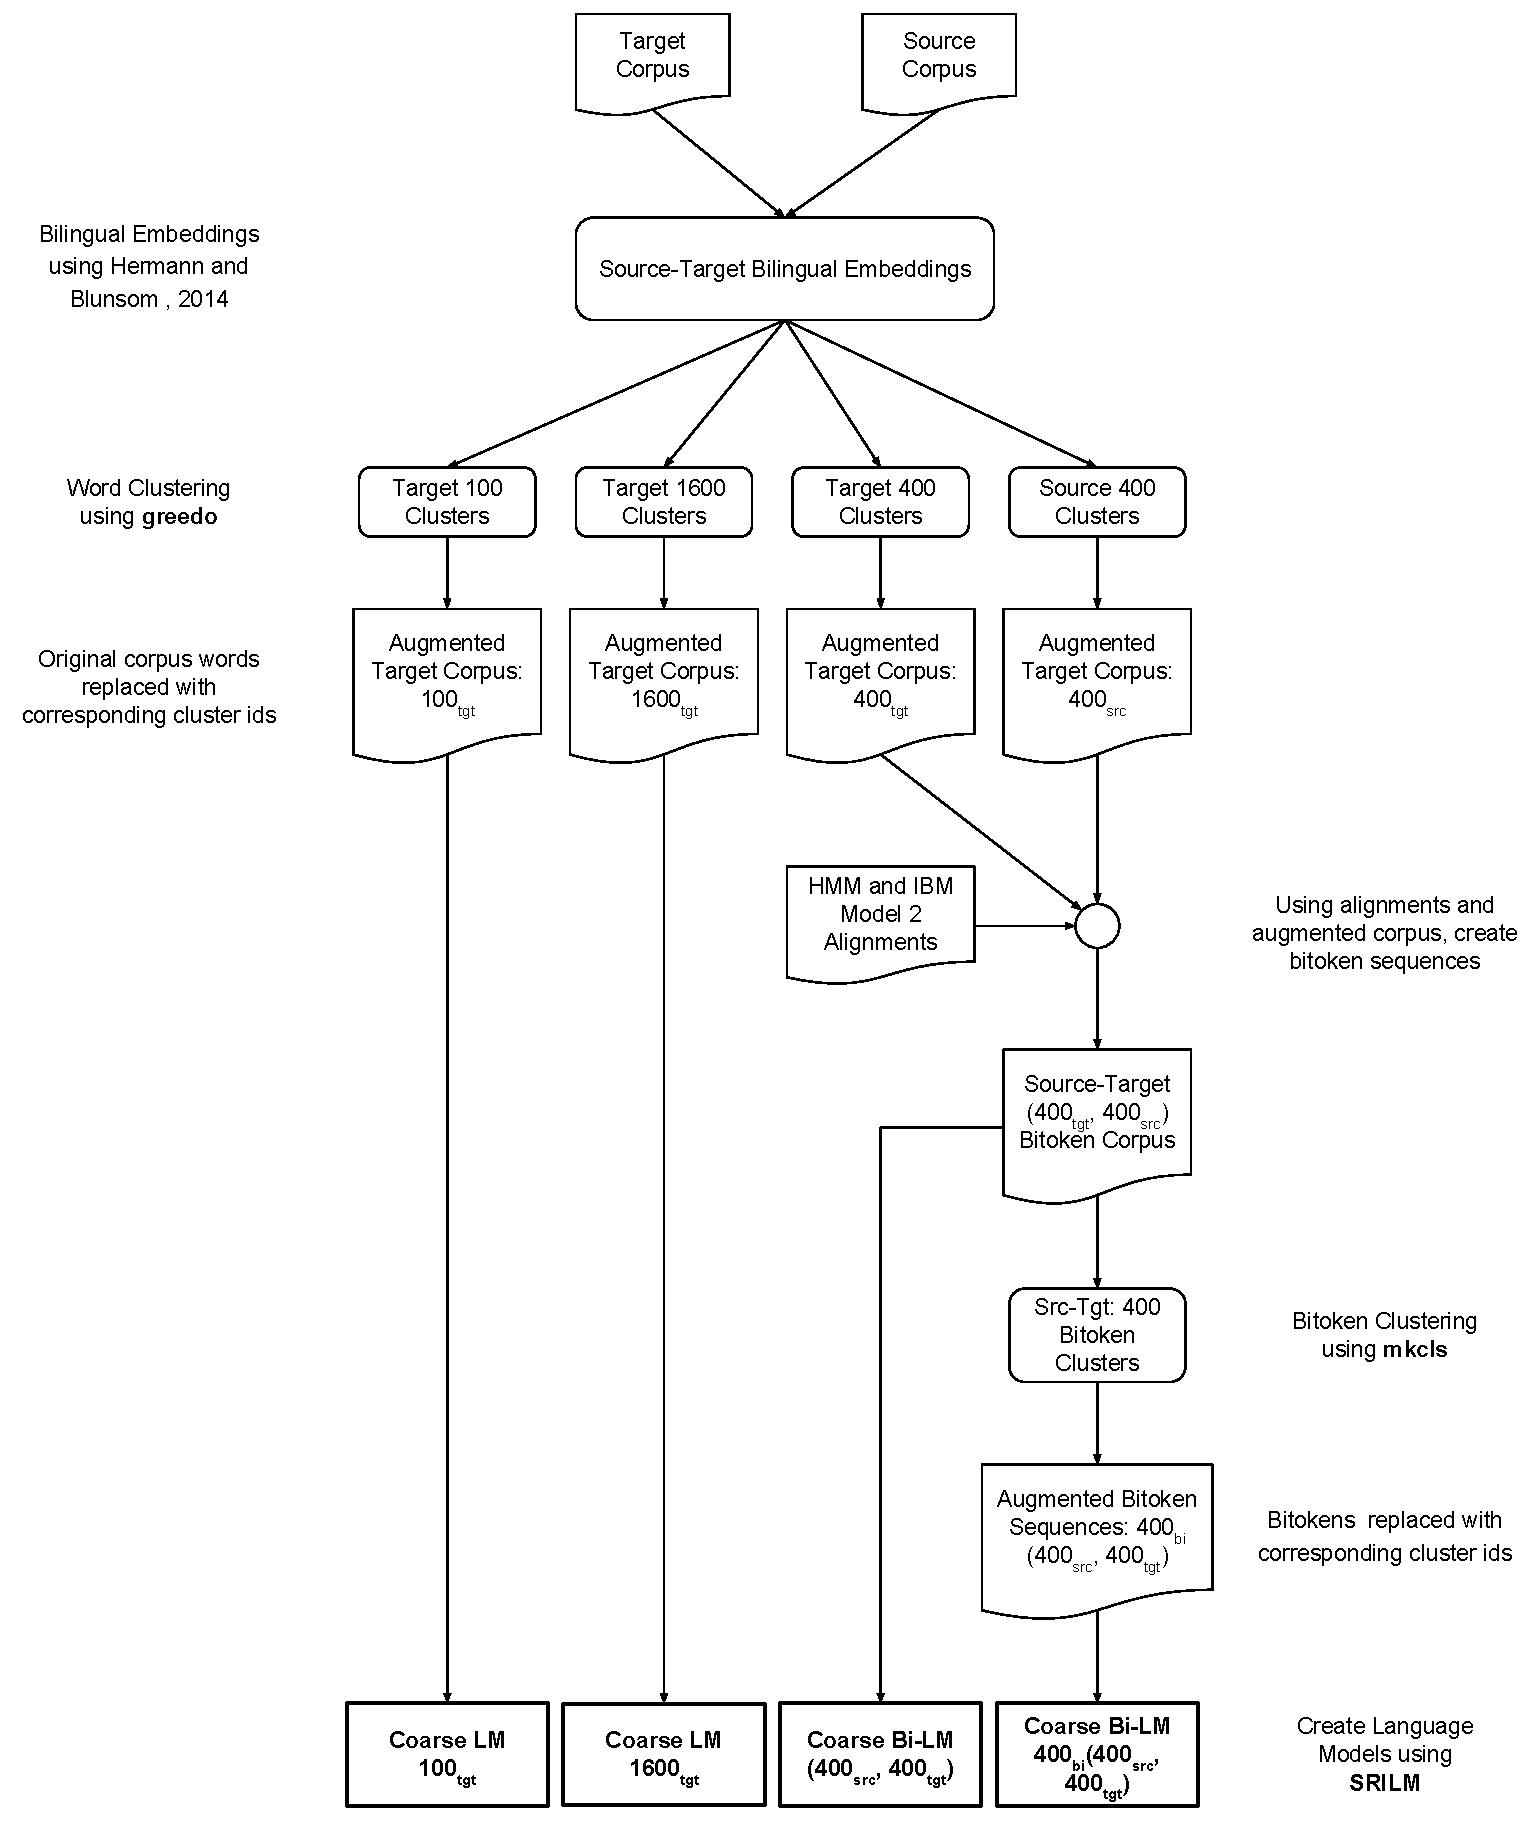
\includegraphics[width=\textwidth]{files/images/idea1}
	\end{center}
	\caption{Approach 1 for creating Coarse LMs and Coarse Bi-LMs}
	\label{fig:idea1}
\end{figure}

\subsubsection{Approach 2}\label{approach2}
Figure~\ref{fig:idea2} shows our second idea to create coarse LMs and Bi-LMs. Based on Approach 1~\ref{approach1}, we first create bilingual word embeddings using \cite{Hermann14} for the sentence aligned parallel corpus used for training the SMT system. The bilingual word embeddings are clustered using \textbf{greedo} to create the same clusters as in Approach 1, which are:
\begin{itemize}
	\item Target language word embedding clusters of size 100, 400 and 1600.
	\item Source language word embeddings cluster of size 400.
\end{itemize}

The clusters are then used to augment the source and target language corpus by replacing the words with their cluster ids. Augmented target language corpus \textit{$100_{tgt}$} and \textit{$1600_{tgt}$} are used to estimate coarse LMs \textit{Coarse LM $100_{tgt}$} and \textit{Coarse LM $1600_{tgt}$}. Augmented corporas \textit{$400_{tgt}$} and \textit{$400_{src}$} along with bidirectional word alignments of the original corpora are used to create bitoken sequences \textit{($400_{src},\ 400_{tgt}$)}. \textit{Coarse Bi-LM $(400_{src},\ 400_{tgt})$} is estimated using the bitoken sequences.

Using \textbf{word2vec}~\cite{Mikolov2013a}, we create bitoken embeddings for bitoken sequence corpus \textit{$(400_{src}, 400_{tgt})$}. As in our baseline system (Figure~\ref{fig:baseline}) and approach 1 (Figure~\ref{fig:idea1}) we had clustered the bitoken sequences using \textbf{mkcls}, we again create clusters of size \textit{400} by clustering the bitoken embeddings using \textbf{greedo}. The bitokens in bitoken sequence corpus \textit{$(400_{src},\ 400_{tgt})$} are replaced with their cluster ids from \textbf{greedo}. The augmented bitoken sequences \textit{$400_{bi}(400_{src},\ 400_{tgt})$} are used to estimate coarse Bi-LM \textit{Coarse Bi-LM $400_{bi}(400_{src},\ 400_{tgt})$} using \textbf{SRILM}.

\begin{figure}[htbp]
	\begin{center}
		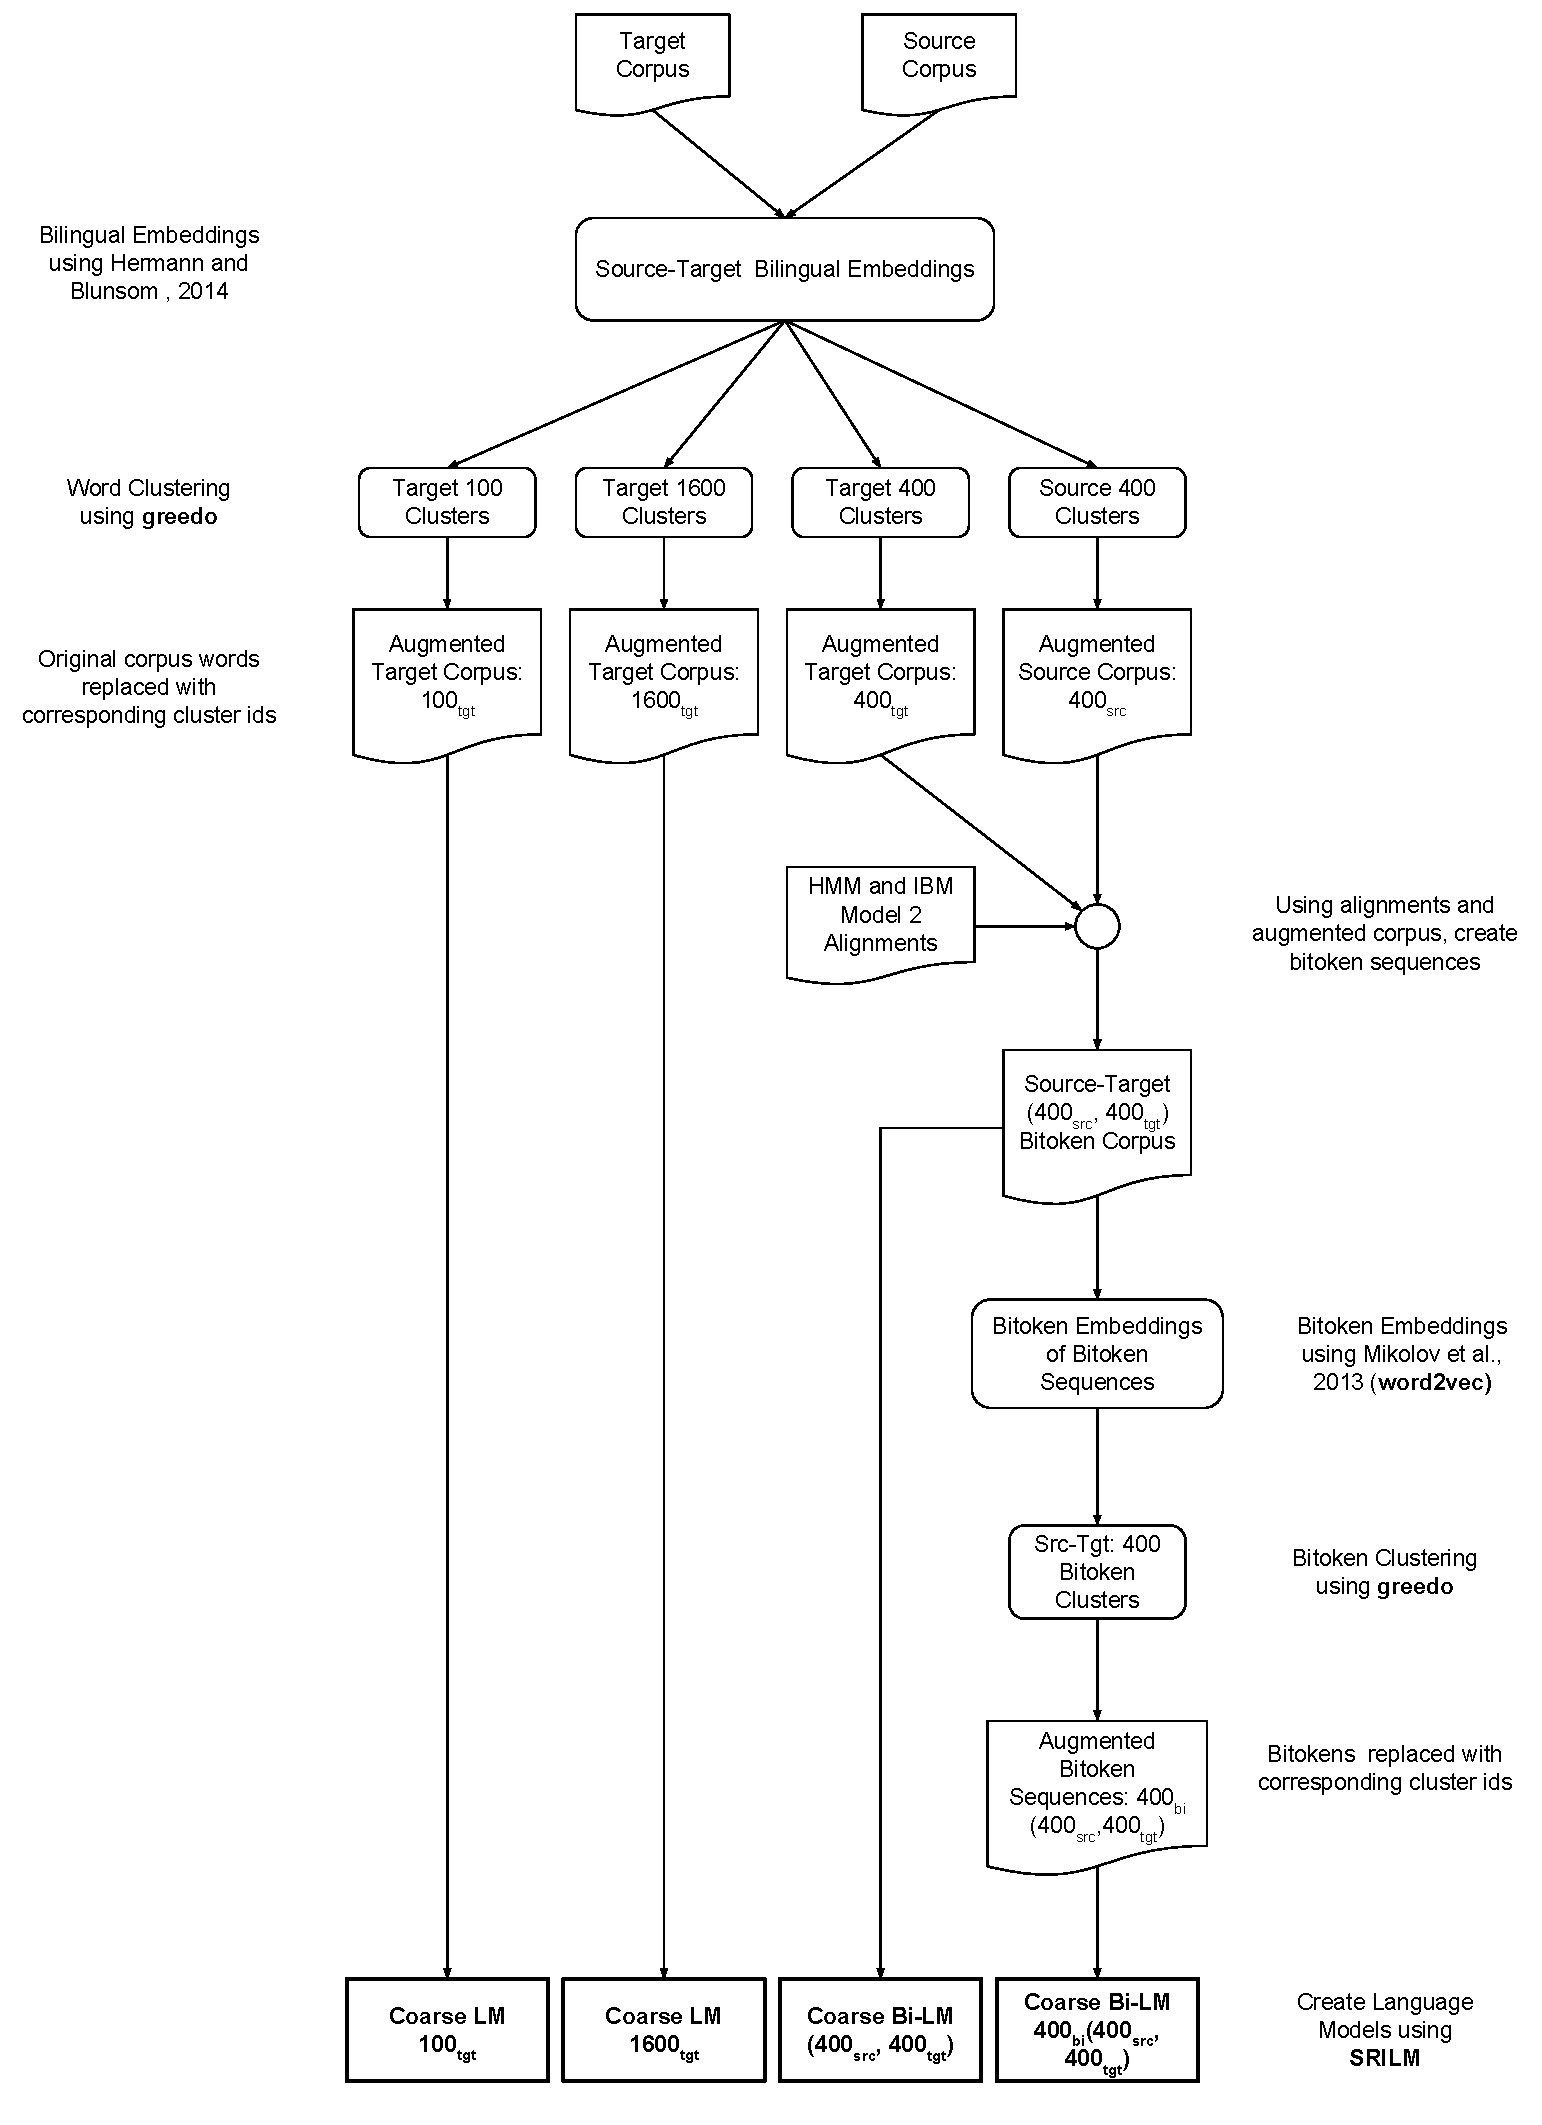
\includegraphics[width=\textwidth]{files/images/idea2}
	\end{center}
	\caption{Approach 2 for creating Coarse LMs and Coarse Bi-LMs}
	\label{fig:idea2}
\end{figure}

\subsubsection{Approach 3}\label{approach3}
In approach 3 (shown in Figure~\ref{fig:idea3}), we estimate the coarse LMs \textit{Coarse LM $100_{tgt}$} and \textit{Coarse LM $1600_{tgt}$} using the same procedure as in approach 1 (\ref{approach1}) and approach 2 (\ref{approach2}).

To create coarse Bi-LM, we first create bitoken sequences using the original sentence aligned parallel corpus along with their alignments. Note, we did not cluster the data before creating the bitoken sequences. Using \textbf{word2vec}, we create bitoken embeddings from the bitoken sequences. The bitoken embeddings are clustered using \textbf{greedo}, with the number of clusters being 400, as done in previous approaches. The bitokens in bitoken sequences are replaced with their corresponding cluster ids to create an augmented corpus \textit{$400_{bi}(|V|_{src},\ |V|_{tgt}$)}. Here \textit{$|V|_{tgt}$} denotes the vocabulary size of target language corpus and \textit{$|V|_{src}$} is the vocabulary size of source language corpus. \textbf{SRILM} is then utilized to estimate \textit{Coarse Bi-LM $400_{bi}(|V|_{src},\ |V|_{tgt})$} using the augmented bitoken corpus \textit{$400_{bi}(|V|_{src},\ |V|_{tgt})$}.

As compared to baseline, approach 1 and approach 2, approach 3 only has one coarse Bi-LM while others have two.

\begin{figure}[htbp]
	\begin{center}
		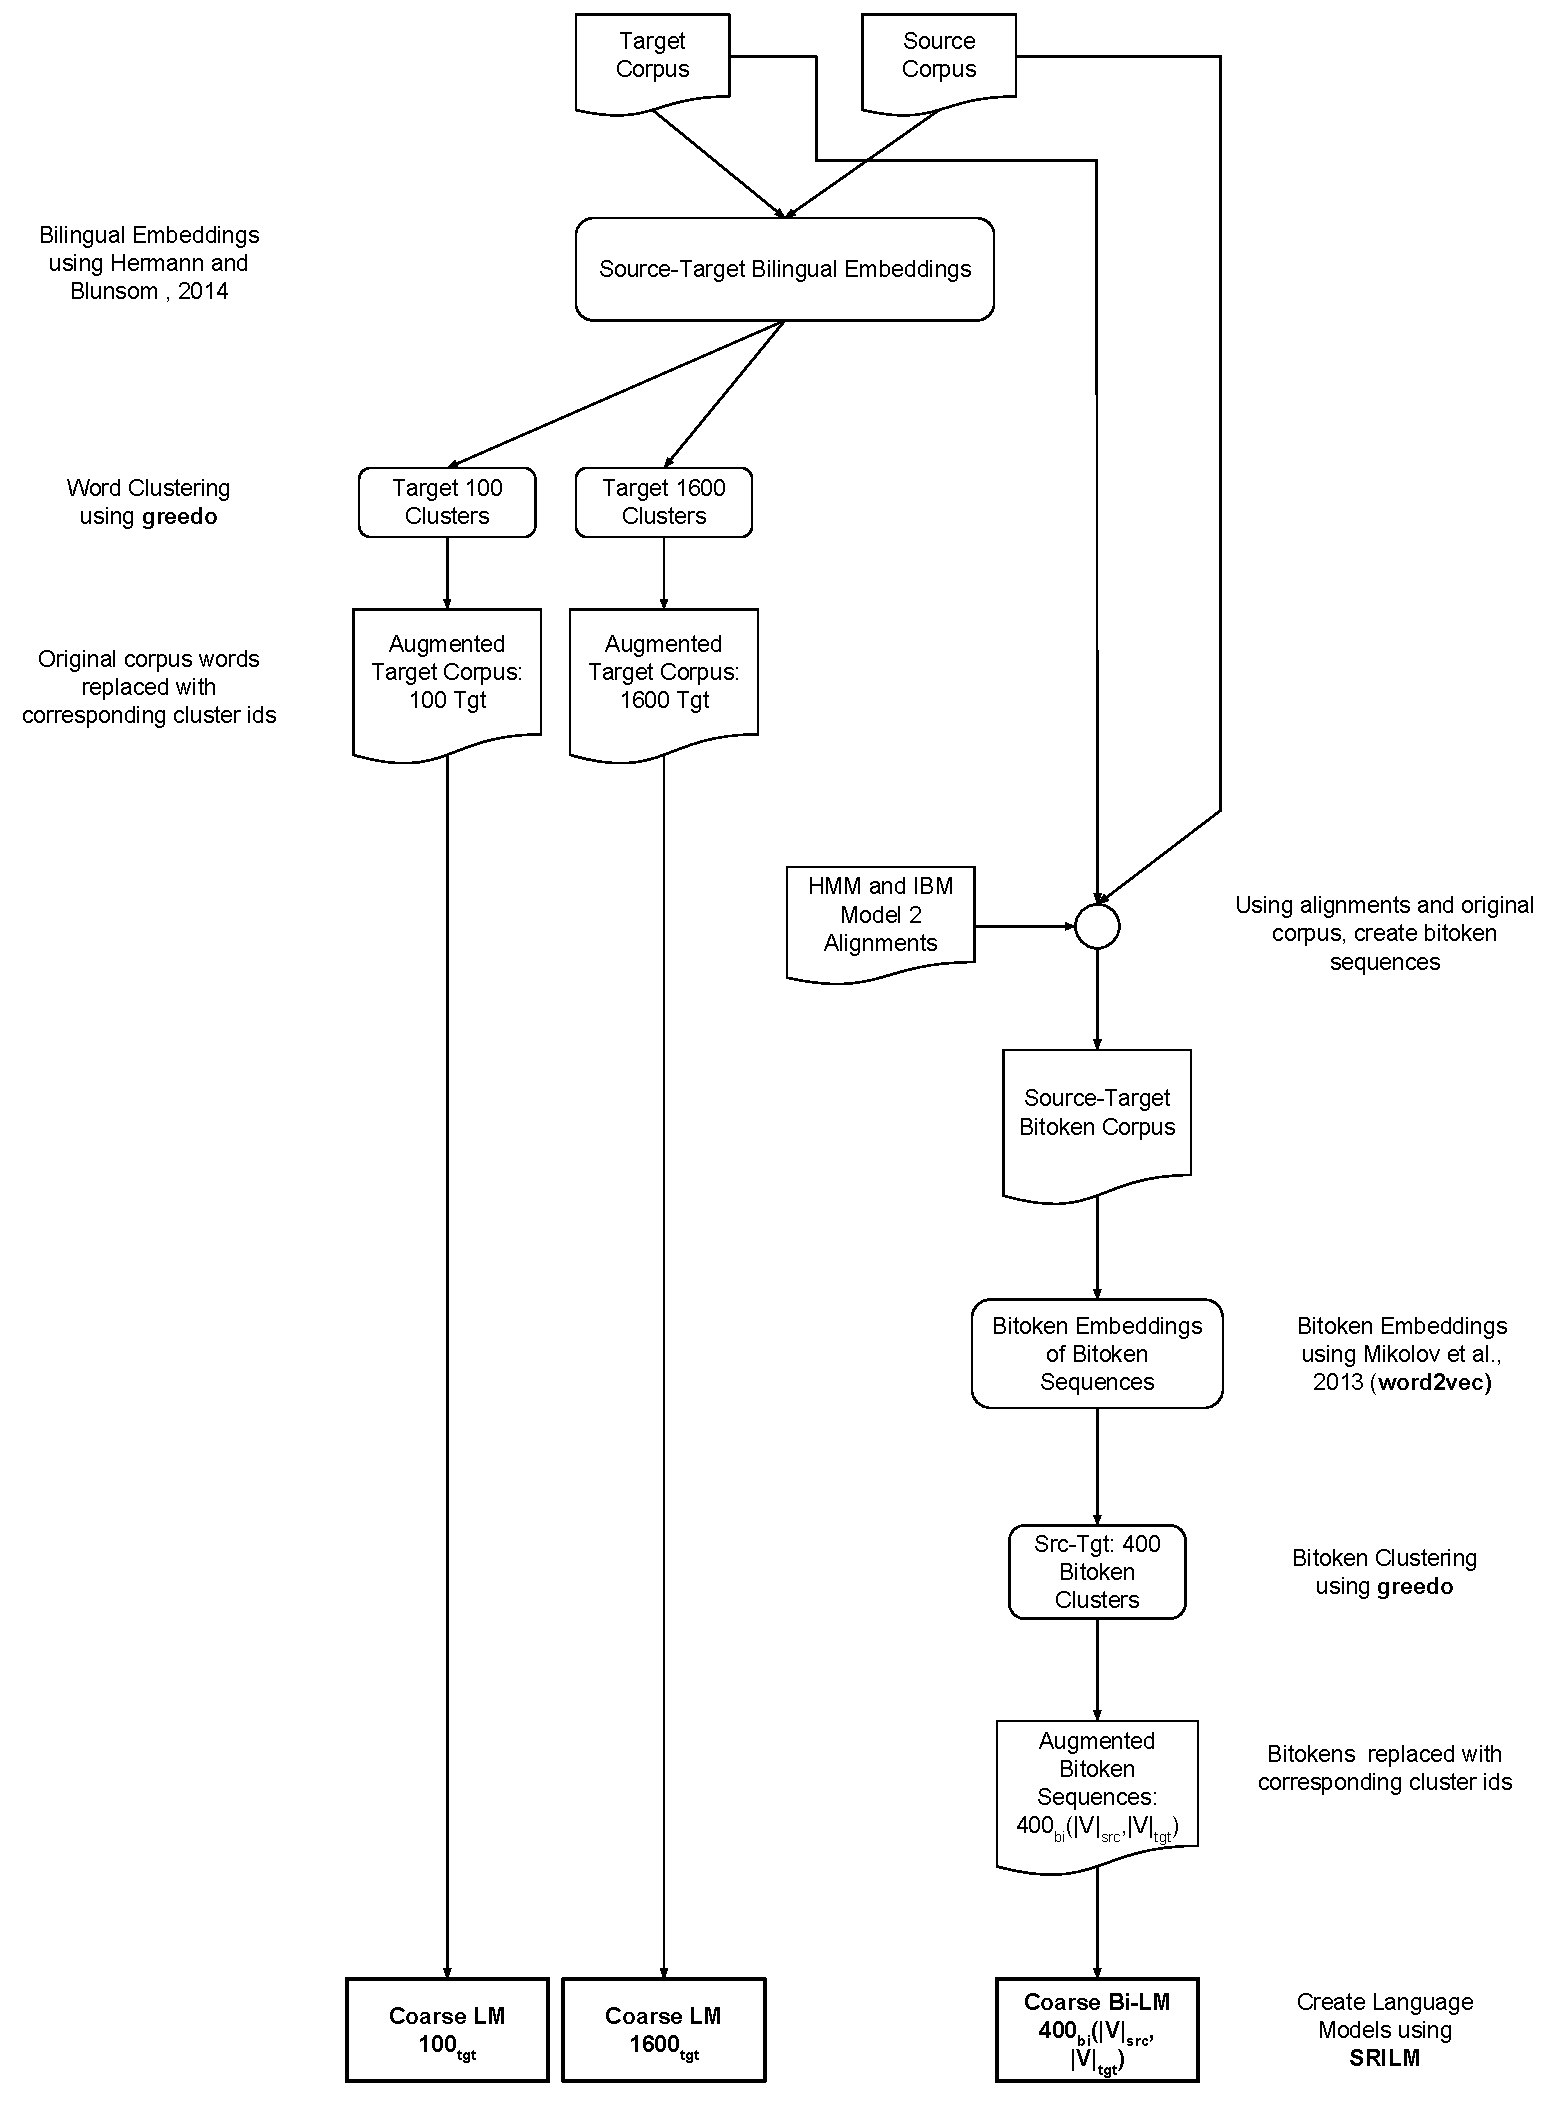
\includegraphics[width=\textwidth]{files/images/idea3}
	\end{center}
	\caption{Approach 3 for creating Coarse LMs and Coarse Bi-LMs}
	\label{fig:idea3}
\end{figure}

%\begin{figure}[htbp]
%	\begin{center}
%		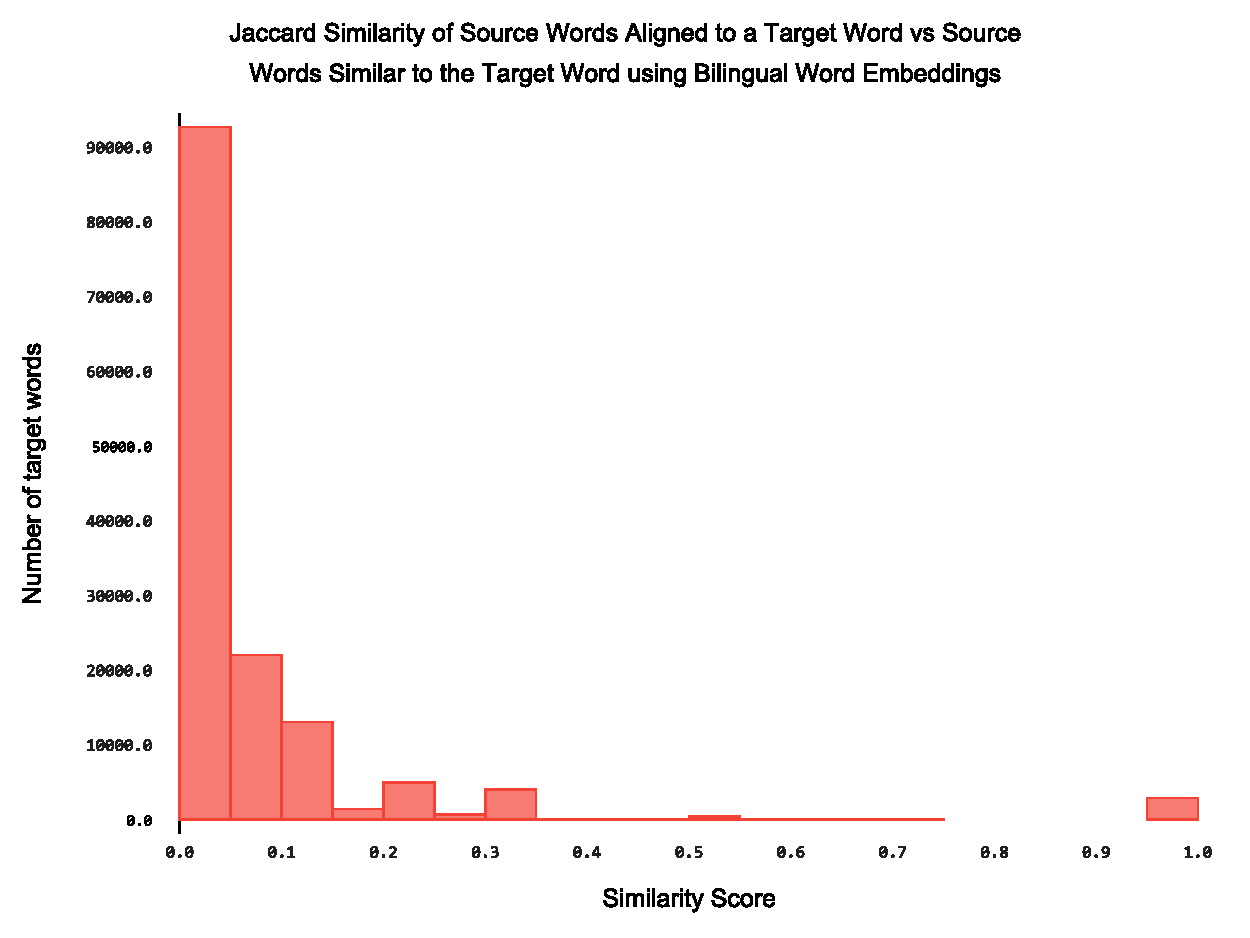
\includegraphics[width=15cm]{files/images/jaccard}
%	\end{center}
%	\caption{Jaccard similarity of source words aligned to each target word using bidirectional alignments and source words similar to the corresponding target words from bilingual word embeddings.}
%	\label{fig:jaccard}
%\end{figure}

In Chapter~\ref{three} we will discuss about the setup and how the three approaches were tested and compare the performance of the three approaches to the baseline system. In the next section we discuss about other approaches in the literature for introducing information about source words.

\section{Previous Work}
In the previous section we introduced Bi-LMs~\cite{Niehues2011,Stewart2014} and three new approaches to estimate coarse LMs and Bi-LMs. Apart from Bi-LMs, there are other approaches for introducing source side contextual information in SMT. \cite{Casacuberta2004} proposed to use stochastic finite state transducers based on bilingual n-grams. This approach was extended by \cite{Marino2006,Crego2010,Zhang2013}. \cite{Allauzen2010} successfully applied the implementation of \cite{Marino2006} on their French-English SMT task. In this approach, the translation model is implemented as a stochastic finite state transducer trained as an n-gram language model of \textit{(source, target)} pairs. When this model is trained, the source sentences are first reordered to match the order of target words using a finite state reordering model. The reordering model uses part-of-speech information to generalize reordering patterns.

\cite{Zhao2005} proposed spectral bilingual clustering for HMM (hidden markov model) based SMT~\cite{Och2003}. This model adds information of both source and target languages to the HMM model. \cite{Hasan2008} introduced a lexical trigger model for SMT in which they used triplets incorporating long distance dependencies that go beyond the local context of phrases and n-gram based language models. \cite{Feng2014} proposed factored markov backoff models along with a robust smoothing strategy that helps to generalize well. \cite{Durrani2011,Durrani2014} proposed \textit{operational sequence models (OSD)} in which they generate a sequence of source and target words and perform reordering by integrating both translation and reordering models into a single generative story. In this approach, translation decisions can influence and get impacted by reordering decisions and vice versa. This approach can be viewed as an extension to \cite{Casacuberta2004,Marino2006}.

\section{Summary}
In this chapter we introduced coarse language models and bilingual language models. We gave an in depth explaination of how bilingual language models are generated using parallel corpus and the alignments between the source and target words. We introduced the work of \cite{Niehues2011} in which he introduced part-of-speech based coarse Bi-LMs which was extended by \cite{Stewart2014} to introduce word class based coarse LMs and coarse Bi-LMs. Motivated by these approaches, we introduced our three approaches to create coarse LMs and Bi-LMs using monolingual embeddings from \textbf{word2vec}~\cite{Mikolov2013a} and bilingual word embeddings~\cite{Hermann14}. As \cite{Stewart2014} had used \textbf{mkcls} to cluster the source and target parallel corpus, we utilized \textbf{greedo}~\cite{Stratos2014} to cluster the word embeddings. Sine, both \textbf{mkcls} and \textbf{greedo} are based on the \cite{Brown1992} model of hierarchical clustering of words, this allows us to compare our approaches more coherently. In the next chapter we discuss about the setup and how we tested the three approaches and compared them to our baseline implementation of \cite{Stewart2014}.

